\documentclass[submit]{harvardml}

% Put in your full name and email address.
\name{Christopher Hase}
\email{christopher\_hase@g.harvard.edu}

% List any people you worked with.
\collaborators{%
  None
}

% You don't need to change these.
\course{CS281-F17}
\assignment{Assignment \#2 v 1.1}
\duedate{5:00pm October 9, 2017}

\usepackage{url, enumitem}
\usepackage{amsfonts}
\usepackage{listings}
\usepackage{bm}
\usepackage{bbm}

\usepackage{hyperref}
\usepackage{tikz}
\usetikzlibrary{bayesnet}
% Some useful macros.
\newcommand{\given}{\,|\,}
\newcommand{\R}{\mathbb{R}}
\newcommand{\E}{\mathbb{E}}
\newcommand{\var}{\text{var}}
\newcommand{\cov}{\text{cov}}
\newcommand{\N}{\mathcal{N}}
\newcommand{\ep}{\varepsilon}

\newcommand{\Dir}{\text{Dirichlet}}
\newcommand{\Bet}{\text{Beta}}
\newcommand{\Ber}{\text{Bernoulli}}
% Useful macros.
\newcommand{\trans}{\mathsf{T}}
\newcommand{\bx}{\mathbf{x}}
\newcommand{\by}{\mathbf{y}}
\newcommand{\bw}{\mathbf{w}}
\newcommand{\distNorm}{\mathcal{N}}
\newcommand{\bzero}{\mathbf{0}}
\newcommand{\ident}{\mathbb{I}}
\renewcommand{\v}[1]{\mathbf{#1}}

\begin{document}


\noindent \textbf{NOTE:} you must show derivations for your answers unless a question explicitly mentions that no justification is required.

%%%%%%%%%%%%%%%%%%%%%%%%%%%%%%%%%%%%%%%%%%%%%%%%%%%%%%%%
%%%%%%%%%%%%%%%%% PROBLEM 1 %%%%%%%%%%%%%%%%%%%%%%%%%%%%
%%%%%%%%%%%%%%%%%%%%%%%%%%%%%%%%%%%%%%%%%%%%%%%%%%%%%%%%
\begin{problem}[Spherical Gaussian, 10pts]
One intuitive way to summarize a probability density is via the mode,
as this is the ``most likely'' value in some sense.  A common example
of this is using the maximum \textit{a posteriori} (MAP) estimate of a
model's parameters.  In high dimensions, however, the mode becomes
less and less representative of typical samples.  Consider variates
from a~$D$-dimensional zero mean spherical Gaussian with unit
variance:
\begin{align*}
  \bx &\sim \distNorm(\bzero_D, \ident_D),
\end{align*}
where~$\bzero_D$ indicates a column vector of~$D$ zeros and~$\ident_D$
is a~${D\times D}$ identity matrix.
\begin{enumerate}
  \item Compute the distribution that this implies over the distance
    of these points from the origin.  That is, compute the
    distribution over~$\sqrt{\bx^\trans\bx}$, if~$\bx$ is a
    realization from~$\distNorm(\bzero_D, \ident_D)$.  (Note: Consider
    transformations of a Gamma distribution described in Murphy 2.4.5.)
  \item Make a plot that shows this probability density function for
    several different values of~$D$, up to ~${D=100}$.

  \item Make a plot of the cumulative distribution function (CDF) over
    this distance distribution for~${D=100}$.  A closed-form solution
    may be difficult to compute, so you can do this numerically.)

  \item From examining the CDF we can think about where most of the
    mass lives as a function of radius.  For example, most of the mass
    for~${D=100}$ is within a thin spherical shell.  From eyeballing
    the plot, what are the inner and outer radii for the shell that
    contains 90\% of the mass in this case?
\end{enumerate}
\end{problem}


\textbf{(a)} $\mathbf{x}=\big[X_1,...,X_D\big]^T$. Using properties of the multivariate normal, we know that $X_i\stackrel{i.i.d.}{\sim}\N(0,1)$. Then, note that $\sqrt{\mathbf{x}^T\mathbf{x}}=\sqrt{\displaystyle\sum_{i=1}^{D}X_i^2}$. First we'll find the distribution of $Y_i=X_i^2$ with support $[0, \infty)$.\\\\\\
$P(Y_i<y_i)=P(X_i^2<y_i)=P(-\sqrt{y_i}<X_i<\sqrt{y_i})$\\\\
$=2P(X_i<\sqrt{y_i})-1=2\Phi(\sqrt{y_i})-1$ (by symmetry of the normal distribution; $\Phi$ is the standard normal CDF)\\\\
$\dfrac{d\big(2\Phi(\sqrt{y_i})-1\big)}{dy_i}=\phi(\sqrt{y_i})\dfrac{1}{\sqrt{y_i}}$ ($\phi$ is the standard normal PDF)\\\\\\
$=\dfrac{1}{\sqrt{2\pi}}y_i^{-\frac{1}{2}}\exp\bigg(-\dfrac{y_i}{2}\bigg)$\\\\\\
This is the PDF for a $\chi^2$ random variable with $1$ degree of freedom, so $Y_i\sim \chi^2_1\Rightarrow X_i^2\sim \chi^2_1$. Now we need to find the distribution of $Z=\displaystyle\sum_{i=1}^{D}X_i^2$ with support $[0,\infty)$. We can do this using the MGF of $Z$.\\\\
MGF$_Z(t)=\displaystyle\prod_{i=1}^{D}$MGF$_{X_i^2}(t)$\\\\\\
$=\displaystyle\prod_{i=1}^{D}(1-2t)^{-\frac{1}{2}}$\\\\\\
$=(1-2t)^{-\frac{D}{2}}$\\\\
This the the MGF of a $\chi^2$ random variable with $D$ degrees of freedom, so $Z\sim\chi^2_D\Rightarrow\displaystyle\sum_{i=1}^{D}X_i^2\sim\chi^2_D$. Lastly, we need to find the distribution of $W=\sqrt{Z}=\sqrt{\displaystyle\sum_{i=1}^{D}X_i^2}$ with support $[0,\infty)$.\\\\
$P(W<w)=P\big(\sqrt{Z}<w\big)$\\\\
$=P\big(Z<w^2\big)$\\\\
$\dfrac{d\Big(P\big(Z<w^2\big)\Big)}{dw}=2wf_Z(w^2)$\\\\\\
$=\dfrac{2^{1-\frac{D}{2}}w^{D-1}}{\Gamma\big(\frac{D}{2}\big)}\exp\bigg(-\dfrac{w^2}{2}\bigg)$\\\\\\
This is the PDF for a $\chi$ random variable with $D$ degrees of freedom, so $W\sim\chi_D$\\\\
$\Rightarrow\sqrt{\displaystyle\sum_{i=1}^{D}X_i^2}=\sqrt{\mathbf{x}^T\mathbf{x}}\sim\chi_D$ and $f_{\sqrt{\mathbf{x}^T\mathbf{x}}}(x)=\dfrac{2^{1-\frac{D}{2}}x^{D-1}}{\Gamma\big(\frac{D}{2}\big)}\exp\bigg(-\dfrac{x^2}{2}\bigg)$

\newpage
%%%%%%%%%%%%%%%%%%%%%%%%%%%%%%%%%%%%%%%%%%%%%%%%%%%%%%%%
%%%%%%%%%%%%%%%%% PROBLEM 2 %%%%%%%%%%%%%%%%%%%%%%%%%%%%
%%%%%%%%%%%%%%%%%%%%%%%%%%%%%%%%%%%%%%%%%%%%%%%%%%%%%%%%
\begin{problem}[Hurdle Models for Count Data, 10pts]

  In this problem we consider predictive models of count data. For
  instance given information about the student $x$, can we predict how
  often they went to the gym that week $y$? A natural choice is to use a Poisson GLM
  i.e. $y$ conditioned on $x$ is modeled as a Poisson distribution.

  However, in practice, it is common for count data of this form to
  follow a bi-modal distribution over count data. For instance, our
  data may come from a survey asking students how often they went to
  the gym in the past week. Some would do so frequently, some would do
  it occasionally but not in the past week (a random zero), and a
  substantial percentage would never do so.

  When modeling this count data with generalized linear models, we
  may observe more zero examples than expected from our model.
  In the case of a Poisson, the mode of the distribution is the
  integer part of the mean. A Poisson GLM may therefore be inadequate
  when means can be relatively large but the mode of the output is 0. Such data is
  common when many data entries have 0 outputs and many also have much
  larger outputs, so the mode of output is 0 but the overall mean is
  not near 0. This problem is known as \textit{zero-inflation}.

  This problem considers handling zero-inflation with a two-part model called
  a \textit{hurdle model}. One part is a binary model such as a logistic model
  for whether the output is zero or positive. Conditional on a positive output,
  the ``hurdle is crossed'' and the second part uses a truncated model that
  modifies an ordinary distribution by conditioning on a positive
  output. This model can handle both zero inflation and zero
  deflation.

  Suppose that the first part of the process is governed by
  probabilities $p(y > 0\ |\ x) = \pi $ and $p(y = 0\ | \ x) = 1 - \pi$; and the second part
  depends on  $\{y\in \mathbb{Z} \ |\ y > 0\}$ and follows a probability mass
  function $f(y\ |\ \mathbf{x})$ that is truncated-at-zero. The
  complete distribution is therefore:
\begin{align*}
P(y = 0\ |\ x) & = 1- \pi\\
P(y = j\ |\ x) & = \pi \frac{f(j\ |\ \mathbf{x})}{1 - f(0\ | \ \mathbf{x})},\ j=1,2,...
\end{align*}
One choice of parameterization is to use a logistic regression model
for $\pi$: $$\pi = \sigma(\mathbf{x}^\top \mathbf{w}_1)$$ and use a Poisson GLM for $f$ with mean parameters $\lambda$ (see
Murphy 9.3): $$\lambda = \exp(\mathbf{x}^\top \mathbf{w}_2) $$

\begin{enumerate}[label=(\alph*)]
\item Suppose we observe $N$ data samples $\{(x_n, y_n)\}_{n=1}^N$.  Write down the log-likelihood for the hurdle model assuming an unspecified mass function $f$.
Give an maximum likelihood estimation approach for the specified parts of the model.

\item Assume now that we select Poisson distribution for $f$. Show
  that the truncated-at-zero Poisson distribution (as used in the
  hurdle model) is a member of the exponential family.  Give its the
  sufficient statistics, natural parameters and log-partition
  function.

\item What is the mean and variance of a truncated Poisson model with mean parameter $\lambda$? If we observe $n$ i.i.d. samples from a truncated Poisson distribution, what is the maximum likelihood estimate of $\lambda$? (Note: Give an equation which could be solved numerically to obtain the MLE. )

\item  Now assume that we using a hurdle model as a GLM with $f$ as a Poisson distribution. Show that
  this is a valid GLM (exponential family for $y$), derive its log-likelihood, and give its sufficient statistics.

\end{enumerate}
\end{problem}

\newpage

\textbf{(a)} $\mathbf{X}\in\R^{N\times m}$ with $\mathbf{x}_i\in\R^m$ as the $i$th row of $\mathbf{X}$ and $x_{ij}\in\R$ as the $j$th element of $\mathbf{x}_i$.\\\\
$\mathbf{Y}\in\R^N$ with $Y_i$ as the $i$th element in $\mathbf{Y}$. Then $\mathbf{y}$ is an instance of $\mathbf{Y}$ and $y_i$ is an instance of $Y_i$.\\\\
$\mathbf{w}_1\in\R^m$ with $w_{1j}$ as the $j$th element in $\mathbf{w}_1$.\\\\
$\mathbf{w}_2\in\R^m$ with $w_{2j}$ as the $j$th element in $\mathbf{w}_2$.\\\\
$\pi_i=\sigma(\mathbf{x}_i^T\mathbf{w}_1)$ $\forall$ $i\in\{1,...,N\}$.\\\\
$\lambda_i=\exp(\mathbf{x}_i^T\mathbf{w}_2)$ $\forall$ $i\in\{1,...,N\}$.\\\\
$\bm{\pi}\in\R^N$ is a vector with $\pi_i$ as the $i$th element and $\bm{\lambda}\in\R^N$ is a vector with $\lambda_i$ as the $i$th element.\\\\
$f$ is an unspecified PDF.\\\\
$\mathbbm{1}$ is an indicator function that takes the value $1$ when its input is true.\\\\\\
$P(\mathbf{Y}=\mathbf{y};\bm{\pi},\bm{\lambda})=\displaystyle\prod_{i=1}^{N}(1-\pi_i)^{\mathbbm{1}[y_i=0]}\Bigg(\pi_i\dfrac{f(y_i;\lambda_i)}{1-f(0;\lambda_i)}\Bigg)^{1-\mathbbm{1}[y_i=0]}$\\\\\\
$\Rightarrow\log\big(P(\mathbf{Y}=\mathbf{y};\bm{\pi},\bm{\lambda})\big)=\displaystyle\sum_{i=1}^{N}\mathbbm{1}[y_i=0]\log(1-\pi_i)+\big(1-\mathbbm{1}[y_i=0]\big)\log\Bigg(\dfrac{f(y_i;\lambda_i)}{1-f(0;\lambda_i)}\Bigg)+\big(1-\mathbbm{1}[y_i=0]\big)\log(\pi_i)$\\\\\\
$=\displaystyle\sum_{i=1}^{N}\log(\pi_i)+\mathbbm{1}[y_i=0]\log\Bigg(\dfrac{1-\pi_i}{\pi_i}\Bigg)+\big(1-\mathbbm{1}[y_i=0]\big)\log\Bigg(\dfrac{f(y_i;\lambda_i)}{1-f(0;\lambda_i)}\Bigg)$\\\\\\
$=\displaystyle\sum_{i=1}^{N}\log(\sigma(\mathbf{x}_i^T\mathbf{w}_1))+\mathbbm{1}[y_i=0]\log\Bigg(\dfrac{1-\sigma(\mathbf{x}_i^T\mathbf{w}_1)}{\sigma(\mathbf{x}_i^T\mathbf{w}_1)}\Bigg)+\big(1-\mathbbm{1}[y_i=0]\big)\log\Bigg(\dfrac{f(y_i;\lambda_i)}{1-f(0;\lambda_i)}\Bigg)$\\\\\\
$=\displaystyle\sum_{i=1}^{N}-\log\big(1+\exp(\mathbf{x}_i^T\mathbf{w}_1)\big)+\big(1-\mathbbm{1}[y_i=0]\big)\mathbf{x}_i^T\mathbf{w}_1+\big(1-\mathbbm{1}[y_i=0]\big)\log\Bigg(\dfrac{f(y_i;\lambda_i)}{1-f(0;\lambda_i)}\Bigg)$\\\\\\
$\dfrac{\partial\log\big(P(\mathbf{Y}=\mathbf{y};\bm{\pi},\bm{\lambda})\big)}{\partial w_{1j}}=\displaystyle\sum_{i=1}^{n}-\dfrac{x_{ij}\exp(\mathbf{x}_i^T\mathbf{w}_1)}{1+\exp(\mathbf{x}_i^T\mathbf{w}_1)}+\big(1-\mathbbm{1}[y_i=0]\big)x_{ij}$ $\forall$ $j\in\{1,...,m\}$\\\\\\
$\Rightarrow\dfrac{\partial\log\big(P(\mathbf{Y}=\mathbf{y};\bm{\pi},\bm{\lambda})\big)}{\partial\mathbf{w}_1}=\Bigg[\dfrac{\partial\log\big(P(\mathbf{Y}=\mathbf{y};\bm{\pi},\bm{\lambda})\big)}{\partial w_{11}},...,\dfrac{\partial\log\big(P(\mathbf{Y}=\mathbf{y};\bm{\pi},\bm{\lambda})\big)}{\partial w_{1m}}\Bigg]^T$\\\\\\
We want to find $\mathbf{\hat w}_1^{MLE}$. This will be the $\mathbf{w}_1$ that makes the gradient of the log-likelihood with respect to $\mathbf{w}_1$ equal to $\mathbf{0}$. To find this $\mathbf{w}_1$, we can use a gradient ascent method. For example, we could initialize $\mathbf{w}_1^{(0)}$ and then use:\\\\
$\mathbf{w}_1^{(i+1)}\leftarrow\mathbf{w}_1^{(i)}+\alpha\dfrac{\partial\log\big(P(\mathbf{Y}=\mathbf{y};\bm{\pi},\bm{\lambda})\big)}{\partial\mathbf{w}_1}\big(\mathbf{w}_1^{(i)}\big)$ until convergence ($\alpha\in\R$ is the learning rate).\\\\\\

\textbf{(b)} Let $Y$ be truncated-at-zero Poisson distributed with parameter $\lambda$.\\\\
$P(Y=y;\lambda)=\dfrac{\frac{\exp(-\lambda)\lambda^y}{y!}}{1-\exp(-\lambda)}$\\\\\\
$=\exp\big(-\lambda+y\log(\lambda)-\log(y!)-\log(1-\exp(-\lambda)\big)$\\\\
$=(y!)^{-1}\exp\Big(y\log(\lambda)-\big(\lambda+\log(1-\exp(-\lambda)\big)\Big)$\\\\\\
$\theta=\log(\lambda)$\\\\
$A(\theta)=\exp(\theta)+\log\big(1-\exp(-\exp(\theta)\big)$\\\\
$\phi(y)=y$\\\\
$h(y)=(y!)^{-1}$\\\\
$\theta$ is the natural parameter, $A(\theta)$ is the log-partition function, $\phi(y)$ is the sufficient statistic, and $h(y)$ is the scaling constant. Because we can write the truncated-at-zero Poisson PMF can be written in the form\\ $P(Y=y;\lambda)=h(y)\exp\big(\theta\phi(y)-A(\theta)\big)$, we know that the truncated-at-zero Poisson distribution is a member of the exponential family.\\\\\\

\textbf{(c)} Let $Y\sim$ Pois$(\lambda)$ and $Y_{trunc}$ be truncated-at-zero Poisson distributed with parameter $\lambda$.\\\\
$E(Y_{trunc})=\displaystyle\sum_{y=0}^{\infty}yP(Y_{trunc}=y)$\\\\
$\Rightarrow\big(1-\exp(-\lambda)\big) E(Y_{trunc})=\displaystyle\sum_{y=0}^{\infty}yP(Y=y)=\lambda$\\\\
$\Rightarrow E(Y_{trunc})=\dfrac{\lambda}{1-\exp(-\lambda)}$\\\\\\\\
Var$(Y_{trunc})=E(Y_{trunc}^2)-\big[E(Y_{trunc})\big]^2$\\\\\\
We'll need to solve for $E(Y_{trunc}^2)$.\\\\
$E(Y_{trunc}^2)=\displaystyle\sum_{y=0}^{\infty}y^2P(Y_{trunc}=y)$\\\\
$\Rightarrow\big(1-\exp(-\lambda)\big) E(Y_{trunc}^2)=\displaystyle\sum_{y=0}^{\infty}y^2P(Y=y)=$Var$(Y)+\big[E(Y)\big]^2=\lambda+\lambda^2$\\\\\\
$\Rightarrow E(Y_{trunc}^2)=\dfrac{\lambda+\lambda^2}{1-\exp(-\lambda)}$\\\\\\
Plugging this and the expectation for $Y_{trunc}$ in, we get:\\\\ Var$(Y_{trunc})=\dfrac{\lambda+\lambda^2}{1-\exp(-\lambda)}-\dfrac{\lambda^2}{\big(1-\exp(-\lambda)\big)^2}$\\\\\\\\
Now let $Y_i$ follow a truncated-at-zero Poisson distribution with parameter $\lambda$ $\forall$ $i\in\{1,...,n\}$ and let $\mathbf{Y}\in\R^n$ have $Y_i$ as its $i$th element. Then $\mathbf{y}$ is an instance of $\mathbf{Y}$ and $y_i$ is an instance of $Y_i$.\\\\
$P(\mathbf{Y}=\mathbf{y};\lambda)=\displaystyle\prod_{i=1}^{n}\dfrac{\frac{\exp(-\lambda)\lambda^y_i}{y_i!}}{1-\exp(-\lambda)}$\\\\\\
$\Rightarrow\log\big(P(\mathbf{Y}=\mathbf{y};\lambda)\big)=\displaystyle\sum_{i=1}^{n}-\lambda+y_i\log(\lambda)-\log(y_i!)-\log(1-\exp(-\lambda)\big)$\\\\\\
$=-n\lambda-n\log\big(1-\exp(-\lambda)\big)+n\bar{y}\log(\lambda)-\displaystyle\sum_{i=1}^{n}\log(y_i!)$\\\\\\
$\dfrac{d\log\big(P(\mathbf{Y}=\mathbf{y};\lambda)\big)}{d\lambda}=-n+\dfrac{n}{1-\exp(\lambda)}+\dfrac{n\bar{y}}{\lambda}$\\\\\\
We want to find $\hat\lambda_{MLE}$. This will be the $\lambda$ that makes the derivative of the log-likelihood with respect to $\lambda$ equal to $0$. To find this $\lambda$, we can use a gradient ascent method. For example, we could initialize $\lambda^{(0)}$ and then use:\\\\
$\lambda^{(i+1)}\leftarrow\lambda^{(i)}+\alpha\dfrac{d\log\big(P(\mathbf{Y}=\mathbf{y};\lambda)\big)}{d\lambda}\big(\lambda^{(i)}\big)$ until convergence ($\alpha\in\R$ is the learning rate).\\\\\\\\


\textbf{(d)} $f(y_i;\lambda_i)=\dfrac{\exp(-\lambda_i)\lambda_i^{y_i}}{y_i!}$ with $\lambda_i=\exp(\mathbf{x}_i^T\mathbf{w}_2)$ $\forall$ $i\in\{1,...,n\}$\\\\
The rest of the notation is the same as in part \textbf{(a)}.\\\\\\
$P(Y_i=y_i;\pi_i,\lambda_i)=(1-\pi_i)^{\mathbbm{1}[y_i=0]}\Bigg(\pi_i\dfrac{\frac{\exp(-\lambda_i)\lambda_i^{y_i}}{y_i!}}{1-\exp(-\lambda_i)}\Bigg)^{1-\mathbbm{1}[y_i=0]}$\\\\\\
$=\exp\Big(\mathbbm{1}[y_i=0]\log(1-\pi_i)+\big(1-\mathbbm{1}[y_i=0]\big)\log(\pi_i)\Big)\exp\Big(-\lambda_i\big(1-\mathbbm{1}[y_i=0]\big)+y_i\big(1-\mathbbm{1}[y_i=0]\big)\log(\lambda_i)-\big(1-\mathbbm{1}[y_i=0]\big)\log(y_i!)-\big(1-\mathbbm{1}[y_i=0]\big)\log\big(1-\exp(-\lambda_i)\big)\Big)$\\\\\\\\
$=\exp\Bigg(\mathbbm{1}[y_i=0]\log\bigg(\dfrac{1-\pi_i}{\pi_i}\bigg)+\log(\pi_i)\Bigg)\exp\big(y_i\log(\lambda_i)-\lambda_i-\log(y_i!)\big)\exp\big(\lambda_i\mathbbm{1}[y_i=0]-y_i\mathbbm{1}[y_i=0]\log(\lambda_i)+\mathbbm{1}[y_i=0]\log(y_i!)\big)\exp\bigg(\big(\mathbbm{1}[y_i=0]-1\big)\Big(\log\big(\exp(\lambda_i)-1\big)-\lambda_i\Big)\bigg)$\\\\\\
$=\exp\Bigg(\mathbbm{1}[y_i=0]\log\bigg(\dfrac{1-\pi_i}{\pi_i}\bigg)+\log(\pi_i)\Bigg)\exp\big(y_i\log(\lambda_i)-\lambda_i-\log(y_i!)\big)\exp\big(\lambda_i\mathbbm{1}[y_i=0]-y_i\mathbbm{1}[y_i=0]\log(\lambda_i)+\mathbbm{1}[y_i=0]\log(y_i!)\big)\exp\bigg(\mathbbm{1}[y_i=0]\log\big(\exp(\lambda_i)-1\big)-\lambda_i\mathbbm{1}[y_i=0]-\log\big(\exp(\lambda_i)-1\big)+\lambda_i\bigg)$\\\\\\
The terms $y_i\mathbbm{1}[y_i=0]\log(\lambda_i)$ and $\mathbbm{1}[y_i=0]\log(y_i!)$ will always be equal to $0$, regardless of the value of $y_i$. Continuing, we have:\\\\\\
$=(y_i!)^{-1}\exp\Bigg(\mathbbm{1}[y_i=0]\bigg(\log\bigg(\dfrac{1-\pi_i}{\pi_i}\bigg)+\log\big(\exp(\lambda_i)-1\big)\bigg)+y_i\log(\lambda_i)-\Big(\log\big(\exp(\lambda_i)-1\big)-\log(\pi_i)\Big)\Bigg)$\\\\\\
$=h(y_i)\exp\big(\bm{\theta}^T\bm{\phi}(y_i)-A(\bm{\theta})\big)$\\\\\\
$\bm{\theta}=[\theta_1$, $\theta_2]^T=\Bigg[\log\bigg(\dfrac{1-\pi_i}{\pi_i}\bigg)+\log\big(\exp(\lambda_i)-1\big)$, $\log(\lambda_i)\Bigg]^T$\\\\\\
$=\Bigg[\log\bigg(\dfrac{1-\sigma(\mathbf{x}_i^T\mathbf{w}_1)}{\sigma(\mathbf{x}_i^T\mathbf{w}_1)}\bigg)+\log\Big(\exp\big(\exp(\mathbf{x}_i^T\mathbf{w}_2)\big)-1\Big)$, $\mathbf{x}_i^T\mathbf{w}_2\Bigg]^T$\\\\\\
$=\bigg[\log\Big(\exp\big(\exp(\mathbf{x}_i^T\mathbf{w}_2)\big)-1\Big)-\mathbf{x}_i^T\mathbf{w}_1$, $\mathbf{x}_i^T\mathbf{w}_2\bigg]^T$\\\\\\
$A(\bm{\theta})=\log\Big(\exp(\theta_1)+\exp\big(\exp(\theta_2)\big)-1\Big)$\\\\
$\bm{\phi}(y_i)=[\mathbbm{1}[y_i=0]$, $y_i$]\\\\
$h(y_i)=(y_i!)^{-1}$\\\\
$\bm{\theta}$ represents the the natural parameters, $A(\bm{\theta})$ is the log-partition function, $\bm{\phi}(y_i)$ represents the sufficient statistics, and $h(y_i)$ is the scaling constant. Because we can write the hurdle model PMF for $Y_i$ in the exponential family form $P(Y_i=y_i;\pi_i,\lambda_i)=h(y_i)\exp\big(\bm{\theta}^T\bm{\phi}(y_i)-A(\bm{\theta})\big)$, we know that the hurdle model is a valid GLM.\\\\
Now we need to derive the log-likelihood for the hurdle model GLM. Starting from the final log-likelihood expression in part \textbf{(a)}, we have:\\
$\log\big(P(Y_i=y_i;\pi_i,\lambda_i)\big)=-\log\big(1+\exp(\mathbf{x}_i^T\mathbf{w}_1)\big)+\big(1-\mathbbm{1}[y_i=0]\big)\mathbf{x}_i^T\mathbf{w}_1+\big(1-\mathbbm{1}[y_i=0]\big)\log\Bigg(\dfrac{\frac{\exp(-\lambda_i)\lambda_i^{y_i}}{y_i!}}{1-\exp(-\lambda_i)}\Bigg)$\\\\
$=-\log\big(1+\exp(\mathbf{x}_i^T\mathbf{w}_1)\big)+\big(1-\mathbbm{1}[y_i=0]\big)\mathbf{x}_i^T\mathbf{w}_1+\big(1-\mathbbm{1}[y_i=0]\big)\Big(y_i\log(\lambda_i)-\big(\lambda_i+\log\big(1-\exp(-\lambda_i)\big)\big)-\log(y_i!)\Big)$
$=-\log\big(1+\exp(\mathbf{x}_i^T\mathbf{w}_1)\big)+\big(1-\mathbbm{1}[y_i=0]\big)\mathbf{x}_i^T\mathbf{w}_1+\big(1-\mathbbm{1}[y_i=0]\big)\Big(y_i\mathbf{x}_i^T\mathbf{w}_2-\big(\exp(\mathbf{x}_i^T\mathbf{w}_2)+\log\big(1-\exp(-\exp(\mathbf{x}_i^T\mathbf{w}_2))\big)\big)-\log(y_i!)\Big)$


%%%%%%%%%%%%%%%%%%%%%%%%%%%%%%%%%%%%%%%%%%%%%%%%%%%%%%%%
%%%%%%%%%%%%%%%%% PROBLEM 3  %%%%%%%%%%%%%%%%%%%%%%%%%%%
%%%%%%%%%%%%%%%%%%%%%%%%%%%%%%%%%%%%%%%%%%%%%%%%%%%%%%%%

\begin{problem}[Directed Graphical and  Naive Bayes, 10pts]
\textit{To draw the DGMs for this problem, we recommend using the \texttt{tikzbayesnet} library. For example the following is drawn in \LaTeX:}
\begin{center}


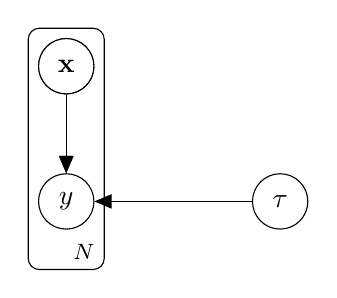
\begin{tikzpicture}
  %Define nodes
  \node[latent]                               (y) {$y$};
  \node[latent, above=of y] (w) {$\mathbf{w}$};
  \node[latent, above=of y]  (x) {$\mathbf{x}$};
  \node[latent, right=2cm of y]            (t) {$\tau$};

  % Connect the nodes
  \edge {x,w,t} {y} ; %

  % Plates
  \plate {yx} {(x)(y)} {$N$} ;

\end{tikzpicture}
\end{center}


\noindent  This problem focuses on modeling a joint distribution of random variables,
$p(y, x_1, \ldots, x_V)$, consisting of discrete variables. These variables represent a class label $y
\in \{1, \ldots, C\}$ and features $x_1 \ldots, x_V$
each of each can take on a values $x_{v} \in \{0, 1\}$.


\begin{enumerate}[label=(\alph*)]
\item  Let $V = 4$. Use the chain rule to select any valid factorization of this joint distribution into univariate distributions. Draw the directed graphical model corresponding to this factorization.

\item What is the sum of the sizes of the \textit{conditional probability tables} associated with
this graphical model. Can you reduce the order of magnitude of this value with a different DGM?

\item  Now consider a naive Bayes factorization of this model, given by,

\[ p(y, x_1, \ldots, x_V ) \approx p(y) \prod_{v} p(x_v | y). \]

Draw a directed graphical model for this factorization.
What is the size of the conditional probability tables required to
fully express any factored distribution of this form?

\item In class, we parameterized naive Bayes such that the class
  distribution is Categorical with a Dirichlet prior, and the
  class-conditional distributions are Bernoulli with a Beta
  prior. Extend the graphical model above to show the generative model
  of $N$ data points and include the parameters and hyper-parameters
  as random variables.


\item Assuming the data obeys the naive Bayes assumptions, answer the following questions as true/false using your directed graphical model.  Justify your answer.

      \begin{itemize}
      \item For a given example, features $x_1$ and $x_2$ are independent.
      \item The class labels $y$ are always conditionally independent of the class-conditional parameters.
      \item Upon observing the class distribution parameters, the class labels are conditionally independent.
      \item Upon observing the class distribution parameters, the features are conditionally independent.
      \item Upon observing the class distribution hyper-parameters, the class labels are conditionally independent.
      \end{itemize}


    \item For the next problem, we will utilize naive Bayes for a
      problem where each example has a \textit{bag} or multiset of
      items. A bag is a set that may contain multiple instances of the
      same value. One approach is to ignore this property and use
      $x_v$ as an indicator function for each item type. An
      alternative is to model $x_v$ with sample space
      $\{0,\ldots, D\}$, where $D$ is the maximum times an item
      appears and to use a Dirichlet-Categorical for the
      class-conditional.  Give one benefit and one drawback of this
      approach. Propose a third option for modeling this distribution.

\end{enumerate}
\end{problem}


\textbf{(a)} $N$ is the number of data points.\\\\
$P(y,x_1,x_2,x_3,x_4)=P(y|x_1,x_2,x_3,x_4)\cdot P(x_1|x_2,x_3,x_4)\cdot P(x_2|x_3,x_4)\cdot P(x_3|x_4)\cdot P(x_4)$
\begin{center}
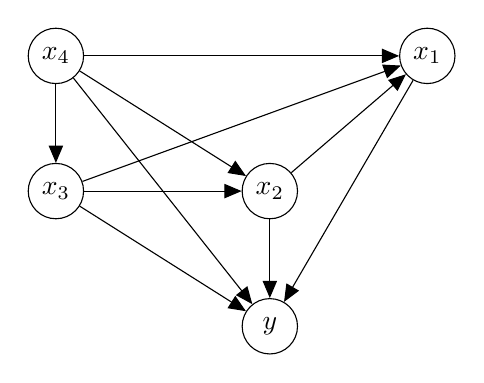
\begin{tikzpicture}
  %Define nodes
  \node[latent] (y) {$y$};
  \node[latent, above= of y]  (x2) {$x_2$};
  \node[latent, left=2cm of x2] (x3) {$x_3$};
  \node[latent, above=of x3] (x4) {$x_4$};
  \node[latent, right=4cm of x4] (x1) {$x_1$};

  % Connect the nodes
  \edge {x1, x2, x3, x4} {y};
  \edge {x2, x3, x4} {x1};
  \edge {x3, x4} {x2};
  \edge {x4} {x3};

\end{tikzpicture}
\end{center}

\textbf{(b)} The size of the conditional probability tables will be $C\cdot2^4$ for $y|x_1,x_2,x_3,x_4$,  $2^4$ for $x_1|x_2,x_3,x_4$,  $2^3$ for $x_2|x_3,x_4$, $2^2$ for $x_3|x_4$. Then the sum of the sizes of the conditional probability tables will be $C\cdot2^4+2^4+2^3+2^2=16C+28$. The size of the marginal probability table for $x_4$ is $2$, so the sum of the sizes of all the probability tables will be $16C+30$.\\\\
Without assuming independence or conditional independence, we cannot reduce the magnitude of this value with a different DGM. Any valid factorization of the joint PDF into univariate distributions where $y|x_1,x_2,x_3,x_4$ is included in the factorization will necessarily yield the same sized conditional probability tables if we do not make independence or conditional independence assumptions.\\\\

\textbf{(c)} $X_1|Y,...,X_V|Y$ are independent. Then the DGM can be represented by the following graph:
\begin{center}
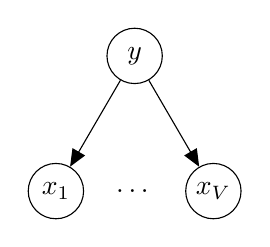
\begin{tikzpicture}
  %Define nodes
  \node[latent] (y) {$y$};
  \node[latent, below=of y, xshift=-1cm]  (x1) {$x_1$};
  \node[latent, below=of y, xshift=1cm]  (xv) {$x_V$};

  % Connect the nodes
  \edge {y} {x1};
  \edge {y} {xv};
  
  \path (x1) -- node[auto=false]{\ldots} (xv);

\end{tikzpicture}
\end{center}
Each conditional probability table will be size $2C$, so the sum of the sizes of the conditional probability tables will be $2CV$. The size of the marginal probability table for $y$ is $C$, so the sum of the sizes of all the probability tables will be $2CV+C$.\\\\

\textbf{(d)} $\theta\sim$ Dir$(\alpha)$ with $\theta,\alpha\in\R^C$. This the prior for the distribution of class labels.\\\\
$Y^{(n)}|\theta\sim$ Cat$(\theta)$ with $Y^{(n)}\in\R^C$ as a one hot encoded vector such that $Y_c^{(n)}=1$ if the $n$th data point has class label $c$ and $0$ otherwise.\\\\
$\beta_{cv}\sim$ Beta$(\beta_{0cv},\beta_{1cv})$ with $\beta_{cv},\beta_{0cv},\beta_{1cv}\in\R$. This is the prior for the $v$th feature for data points that have class label $c$.\\\\
$X_v^{(n)}|\beta_{cv}\sim$ Bern$\big(\beta_{cv}\big)$\\\\\\\\\\\\\\\\
The DGM can then be represented by the following graph:
\begin{center}
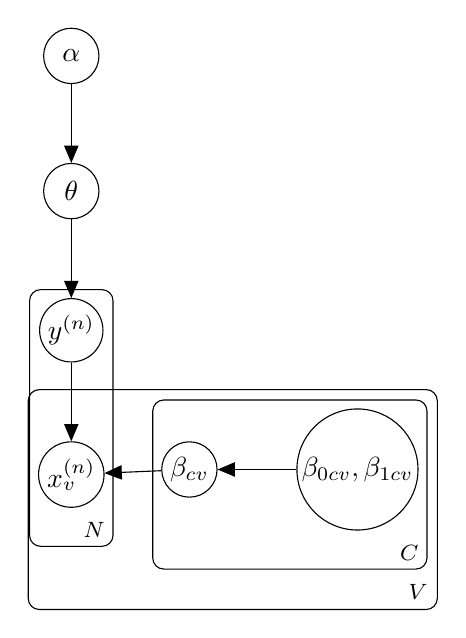
\begin{tikzpicture}
  %Define nodes
  \node[latent] (alpha) {$\alpha$};
  \node[latent, below=of alpha]  (theta) {$\theta$};
  \node[latent, below=of theta]  (y) {$y^{(n)}$};
  \node[latent, below=of y, xshift=1.5cm]  (beta) {$\beta_{cv}$};
  \node[latent, right=1cm of beta]  (betacv) {$\beta_{0cv},\beta_{1cv}$};
  \node[latent, below=of y]  (x) {$x_v^{(n)}$};

  % Connect the nodes
  \edge {alpha} {theta};
  \edge {theta} {y};
  \edge {y} {x};
  \edge {beta} {x};
  \edge {betacv} {beta};
  
  % Plates
  \plate [inner sep =0.1cm] {C} {(betacv)(beta)} {$C$};
  \plate {V} {(x)(C)} {$V$};
  \plate [inner sep = 0.1cm] {N} {(y)(x)} {$N$};
  

\end{tikzpicture}
\end{center}
Note that $\beta_{cv}$ is used to generate $x_v^{(n)}\Leftrightarrow y^{(n)}_c = 1$. Otherwise it is ignored.\\\\

\textbf{(e)}\\\\
\textbf{(1)} False. The path from feature $x_1^{(n)}$ to $x_2^{(n)}$ through $y^{(n)}$ is not blocked.\\\\
\textbf{(2)} False. The path from the class labels to the class-conditional parameters through the features is not blocked when the features are in the evidence.\\\\
\textbf{(3)} True. The path from $y^{(i)}$ to $y^{(j)}$ through $\theta$ is blocked when $\theta$ is in the evidence.\\\\
\textbf{(4)} False. The path from $x_i^{(n)}$ to $x_j^{(n)}$ through $y^{(n)}$ is not blocked when the class distribution parameters are in the evidence.\\\\
\textbf{(5)} False. The path from $y^{(i)}$ to $y^{(j)}$ through $\theta$ is not blocked when $\alpha$ is in the evidence.\\\\\\

\textbf{(f)} A benefit would be that the model captures the fact that there can be multiple instances of each feature in a given example via the class-conditional distributions for each feature. We lose information about a given example by only allowing for binary features. A drawback is that the number of parameters required to fit the model is multiplied by something on the order of $\frac{D}{2}$. As a result, if we don't have a ton of data, we may not be able to achieve a generalizable model fit. A third option would be to model the entire distribution over features for each class using a Dirichlet-Multinomial. This would allow us to capture the fact that there can be multiple instances of each feature in a given example without requiring as many parameters to fit the model.

%%%%%%%%%%%%%%%%%%%%%%%%%%%%%%%%%%%%%%%%%%%%%%%%%%%%%%%%
%%%%%%%%%%%%%%%%% PROBLEM 4 %%%%%%%%%%%%%%%%%%%%%%%%%%%%
%%%%%%%%%%%%%%%%%%%%%%%%%%%%%%%%%%%%%%%%%%%%%%%%%%%%%%%%
\begin{problem}[Naive Bayes Implementation, 10pts]

\noindent You will now implement a naive Bayes classifier for
for sentiment classification. For this problem you will use
the IMDB Movie Reviews dataset which consists of positive and negative movie reviews . Here are two example reviews:\\

        \texttt{there is no story! the plot is hopeless! a filmed based on a car with a \\
        \indent stuck accelerator, no brakes, and a stuck automatic transmission gear \\
        \indent lever cannot be good! ...  i feel sorry for the actors ... poor script ... \\
        \indent heavily over-dramatized ... this film was nothing but annoying, \\
        \indent stay away from it!} [negative review] \\

        \texttt{i had forgotten both how imaginative the images were, and how witty \\
        \indent the movie ... anyone interested in politics or history will love the movie's \\
        \indent offhand references - anyone interested in romance will be moved - this \\
        \indent one is superb.} [positive review] \\

      \noindent As noted in the last problem, it is common to think of
      the input data as a bag/multiset. In text applications,
      sentences are often represented as a \textit{bag-of-words},
      containing how many times each word appears in the sentence. For
      example, consider two sentences:
\begin{itemize}
\item \begin{verbatim}We like programming. We like food.\end{verbatim}
\item \begin{verbatim}We like CS281.\end{verbatim}
\end{itemize}
A vocabulary is constructed based on these two sentences:
\begin{verbatim}
                 ["We", "like", "programming", "food", "CS281"]
\end{verbatim}
Then the two sentences are represented as the number of occurrences of each word in the vocabulary (starting from position 1):
\begin{itemize}
\item \begin{verbatim}[0, 2, 2, 1, 1, 0]\end{verbatim}
\item \begin{verbatim}[0, 1, 1, 0, 0, 1]\end{verbatim}
\end{itemize}

\noindent We have included a utility file \texttt{utils.py} that does this mapping. For
these problems you can therefore treat text in this matrix representation.


\begin{itemize}

	\item Implement a Naive Bayes classifier using a
          Bernoulli class-conditional with a Beta prior
          where each feature is an indicator that
          a word appears at least once in the bag.

    \item Implement a Naive Bayes classifier using a Categorical
          class-conditional with a Dirichlet prior. Here
          the features represent that count of each word in
          the bag.



    \item For both models, experiment with various settings
          for the priors. For the Dirichlet prior on
          the class, begin with $\boldsymbol{\alpha} = \v 1$
          (Laplace Smoothing).
          Do the same for the class-conditional prior
          (be it Dirichlet or Beta). Keeping uniformity,
          vary the magnitude to $.5$ and smaller. If the
          classes are unbalanced in the dataset, does it help
          to use a larger $\alpha$ for the less-often occuring
          class? Optionally, choose class-conditional priors based on an
          outside text source. Validate your choices on the validation set,
          and report accuracy on the test set.

      \item (Optional) With the bag-of-words representation, 
             would the model be able to capture phrases
             like ``don't like''? An alternative to the bag-of-words model is
          known as the bag-of-bigrams model, where a bigram is two
          consecutive words in a sentence.  Modify \texttt{utils.py}
          to include bigram features with either model and see if they
          increase accuracy.

    \item (Optional Reading) \textit{Baselines and Bigrams: Simple, Good Sentiment and Topic Classification}\\
    \url{http://www.aclweb.org/anthology/P/P12/P12-2.pdf#page=118}\\
\end{itemize}
\end{problem}

Test accuracy $=0.864$\\
Class prior parameter magnitude = $1$\\
Beta class-conditional prior parameter magnitude = $1$\\\\
Test accuracy $=0.863$\\
Class prior parameter magnitude = $1$\\
Dirichlet class-conditional prior parameter magnitude = $0.4$\\
Note that the maximum number of times that a feature could be drawn to was set to $D=10$ (see \textbf{3(f)})\\\\
The classes are not unbalanced in the dataset, so increasing the relative value of the prior parameter for the less often occurring class is not a relevant question here. If the classes were imbalanced, it still seems that we would want our prior to reflect the truth. That is, if our goal is to maximize accuracy, we would want our posterior mean for the distribution over classes to reflect the distribution over classes for the data we want to make predictions on, and choosing a prior that reflects the distribution over classes for data we want to make predictions on would help to give us such a posterior mean. If we have a goal for our model for which we care about false positives, false negatives, true positives, and true negatives, then we may want to choose a prior with non-uniformity for the distribution over classes to help us achieve that goal.
 
\newpage
%%%%%%%%%%%%%%%%%%%%%%%%%%%%%%%%%%%%%%%%%%%%%%%%%%%%%%%%
%%%%%%%%%%%%%%%%% PROBLEM 5 %%%%%%%%%%%%%%%%%%%%%%%%%%%%
%%%%%%%%%%%%%%%%%%%%%%%%%%%%%%%%%%%%%%%%%%%%%%%%%%%%%%%%
\begin{problem}[Logistic Regression with Autograd, 15pts]

  In the previous problem, you implemented a Naive Bayes classifier
  for sentiment classification on the IMDB Movie Reviews dataset.  In this
  problem, you will apply logistic regression to the same task.

\begin{enumerate}[label=(\alph*)]

    \item $\ell_1$-regularized logistic regression. Consider a model parameterized by $\mathbf{w}$:
    \begin{align*}
        p(\mathbf{w}) & = \frac{1}{2b}\exp(-\frac{\|\mathbf{w}\|_1}{b}) \\
    p(y = 1 | \mathbf{x}, \mathbf{w}) & = \sigma(\mathbf{w}^\top \mathbf{x})\\
    p(y = 0 | \mathbf{x}, \mathbf{w}) & = 1 - \sigma (\mathbf{w}^\top \mathbf{x})
    \end{align*}
    where $\sigma(\cdot)$ is the
    sigmoid
      function. Note that we are imposing a Laplacian prior on
    $\mathbf{w}$, see Murphy, 2.4.4.

        \begin{enumerate}[label=(\roman*)]
             \item Given a dataset $\{(\mathbf{x}^{(i)},y^{(i)})\}_{i=1}^N$, derive the necessary gradient updates for MAP of $\mathbf{w}$.\footnote{You only need to consider the case where $\forall i, w_i\neq 0$. If $\exists i, w_i=0$, we can use its \href{https://see.stanford.edu/materials/lsocoee364b/01-subgradients_notes.pdf}{subgradients} instead.}
             \item Show that for some constant $\lambda$, MAP inference of $\mathbf{w}$ is equivalent to minimizing
                 \begin{equation*}
                     - \frac{1}{N} \sum_{i=1}^N \log p(y^{(i)}|\mathbf{x}^{(i)},
                     \mathbf{w}) + \lambda \|\mathbf{w}\|_1
                 \end{equation*}
         \end{enumerate}

    \item Implementation using PyTorch automatic differentiation.\footnote{\url{https://github.com/harvard-ml-courses/cs281/blob/master/cs281-f17/sections/04/walkthrough.ipynb}.}
        \begin{enumerate}[label=(\roman*)]
             \item
               Using the bag-of-words feature representation from the previous question, train a logistic regression model using PyTorch autograd and \href{http://pytorch.org/tutorials/beginner/examples_nn/two_layer_net_nn.html}{\texttt{torch.nn}}. Report test accuracy.
                 Select regularization strength $\lambda$ based on validation accuracy.
             \item Which 5 words correspond to the largest weight indices, per class, in the
                   learnt weight vectors? Which 5 words correspond to the least weight
                   indices?
             \item Study how sparsity (i.e percentage of zero elements in a vector)
                 of the parameter vector changes with different values of $\lambda$.
                 Again, tune $\lambda$ on the validation set and report the test accuracies
                 on the test set. Suggested values to try are $\{0,0.001,0.01,0.1,1\}$. You can treat parameters with $<1e-4$ absolute values as zeros.
         \end{enumerate}

\end{enumerate}

\end{problem}


\textbf{(a)(i)} $\mathbf{X}\in\R^{N\times m}$ with $\mathbf{x}_i\in\R^m$ as the $i$th row of $\mathbf{X}$ and $x_{ij}\in\R$ as the $j$th element of $\mathbf{x}_i$.\\\\
$\mathbf{Y}\in\R^N$ with $Y_i$ as the $i$th element in $\mathbf{Y}$. Then $\mathbf{y}$ is an instance of $\mathbf{Y}$ and $y_i$ is an instance of $Y_i$.\\\\
$\mathbf{W}\in\R^m$ with $W_i$ as the $i$th element in $\mathbf{W}$. Then $\mathbf{w}$ is an instance of $\mathbf{W}$ and $w_i$ is an instance of $W_i$.\\\\
$p(\mathbf{w}|\mathbf{y},\mathbf{X})\propto p(\mathbf{y}|\mathbf{X},\mathbf{w})p(\mathbf{w}|\mathbf{X})$\\\\
$=\displaystyle\prod_{i=1}^{N}p(y_i|\mathbf{x}_i,\mathbf{w})p(\mathbf{w}|\mathbf{x}_i)=p(\mathbf{w})^N\displaystyle\prod_{i=1}^{N}p(y_i|\mathbf{x}_i,\mathbf{w})$\\\\\\
$\Rightarrow\log\big(p(\mathbf{y}|\mathbf{X},\mathbf{w})p(\mathbf{w})\big)=\displaystyle\sum_{i=1}^{N}\log\big(p(y_i|\mathbf{x}_i,\mathbf{w})\big)+N\log\big(p(\mathbf{w})\big)$\\\\\\
$=\displaystyle\sum_{i=1}^{N}\log\big(p(y_i|\mathbf{x}_i,\mathbf{w})\big)-\dfrac{N||\mathbf{w}||_1}{b}-N\log(2b)$\\\\\\
From problem \textbf{2(a)}, we know that this simplifies to:\\\\
$=\displaystyle\sum_{i=1}^{N}-\log\big(1+\exp(\mathbf{x}_i^T\mathbf{w})\big)+y_i\mathbf{x}_i^T\mathbf{w}\mathbf-\dfrac{N||\mathbf{w}||_1}{b}-N\log(2b)$\\\\\\
$\dfrac{\partial\big(p(\mathbf{w}|\mathbf{y},\mathbf{X})\big)}{\partial w_j}=\displaystyle\sum_{i=1}^{n}-\dfrac{x_{ij}\exp(\mathbf{x}_i^T\mathbf{w})}{1+\exp(\mathbf{x}_i^T\mathbf{w})}+y_ix_{ij}-\dfrac{Nw_j}{b|w_j|}$ $\forall$ $j\in\{1,...,m\}$ (case where no $w_i=0$)\\\\\\
$\Rightarrow\dfrac{\partial\big(p(\mathbf{w}|\mathbf{y},\mathbf{X})\big)}{\partial \mathbf{w}}=\Bigg[\dfrac{\partial\big(p(\mathbf{w}|\mathbf{y},\mathbf{X})\big)}{\partial w_1},...,\dfrac{\partial\big(p(\mathbf{w}|\mathbf{y},\mathbf{X})\big)}{\partial w_m}\Bigg]^T$\\\\\\
We want to find $\mathbf{\hat w}^{MAP}$. This will be the $\mathbf{w}$ that makes the gradient of the log-likelihood with respect to $\mathbf{w}$ equal to $\mathbf{0}$. To find this $\mathbf{w}$, we can use a coordinate ascent method.\\\\

\textbf{(a)(ii)} Note that $\mathbf{\hat w}^{MAP}$, which is the $\mathbf{w}$ maximizes $\displaystyle\sum_{i=1}^{N}\log\big(p(y_i|\mathbf{x}_i,\mathbf{w})\big)-\dfrac{N||\mathbf{w}||_1}{b}-N\log(2b)$ (we showed this in part \textbf{(a)(i)}) will be the same $\mathbf{w}$ that minimizes $-\dfrac{1}{N}\displaystyle\sum_{i=1}^{N}\log\big(p(y_i|\mathbf{x}_i,\mathbf{w})\big)+\dfrac{||\mathbf{w}||_1}{b}$ since we modified the first expression by negating it, multiplying by a constant, and deleting a term that did not depend on $\mathbf{w}$. Thus, we can find $\mathbf{\hat w}^{MAP}$ by minimizing the following with respect to $\mathbf{w}$:\\\\
$-\dfrac{1}{N}\displaystyle\sum_{i=1}^{N}\log\big(p(y_i|\mathbf{x}_i,\mathbf{w})\big)+\lambda||\mathbf{w}||_1$ where $\lambda=\dfrac{1}{b}$\\\\\\

\textbf{(b)(i)} Validation accuracy when $\lambda=0:$ $0.858$\\
Validation accuracy when $\lambda=0.001:$ $0.819$\\
Validation accuracy when $\lambda=0.01:$ $0.738$\\
Validation accuracy when $\lambda=0.1:$ $0.557$\\
Validation accuracy when $\lambda=1:$ $0.534$\\
Test accuracy when $\lambda=0:$ $0.860$\\\\

\textbf{(b)(ii)}\\\\
Words with highest valued coefficients for predicting class $0$: ['worst' 'bad' 'waste' 'poor' 'nothing']\\\\
Words with lowest valued coefficients for predicting class $0$: ['great' 'best' 'excellent' 'well' 'loved']\\\\
Words with highest valued coefficients for predicting class $1$: ['great' 'best' 'excellent' 'well' 'loved']\\\\
Words with lowest valued coefficients for predicting class $1$: ['worst' 'bad' 'waste' 'poor' 'nothing']\\\\\\

\textbf{(b)(iii)} Validation accuracy when $\lambda=0:$ $0.858$\\
Validation accuracy when $\lambda=0.001:$ $0.819$\\
Validation accuracy when $\lambda=0.01:$ $0.738$\\
Validation accuracy when $\lambda=0.1:$ $0.557$\\
Validation accuracy when $\lambda=1:$ $0.534$\\\\
Test accuracy when $\lambda=0:$ $0.860$\\
Test accuracy when $\lambda=0.001:$ $0.815$\\
Test accuracy when $\lambda=0.01:$ $0.739$\\
Test accuracy when $\lambda=0.1:$ $0.554$\\
Test accuracy when $\lambda=1:$ $0.522$\\\\\\
Number of $0$ valued parameters for class $0$ ($\lambda=0$): $0.0453$\\
Number of $0$ valued parameters for class $1$ ($\lambda=0$): $0.0462$\\\\
Number of $0$ valued parameters for class $0$ ($\lambda=0.001$): $0.9898$\\
Number of $0$ valued parameters for class $1$ ($\lambda=0.001$): $0.9898$\\\\
Number of $0$ valued parameters for class $0$ ($\lambda=0.01$): $0.995$\\
Number of $0$ valued parameters for class $1$ ($\lambda=0.01$): $0.996$\\\\
Number of $0$ valued parameters for class $0$ ($\lambda=0.1$): $0.0995$\\
Number of $0$ valued parameters for class $1$ ($\lambda=0.1$): $0.0982$\\\\
Number of $0$ valued parameters for class $0$ ($\lambda=1$): $0.0424$\\
Number of $0$ valued parameters for class $1$ ($\lambda=1$): $0.0415$\\\\
When we increase $\lambda$ from $0$ to $0.001$, the sparsity of the parameters increases drastically. It increases still for the increase in $\lambda$ from $0.001$ to $0.01$. However, for the increase in $\lambda$ from $0.01$ to $0.1$ we see a huge drop in sparsity. We then see another drop in sparsity when we increase $\lambda$ from $0.1$ to $1$. The increase in sparsity along with increases in $\lambda$ is what we would expect to see. I suspect that the reason that we see the drops in sparsity for the last two increases in $\lambda$ is that stochastic gradient descent never achieves any sort of convergence to a minimum.


\newpage
%%%%%%%%%%%%%%%%%%%%%%%%%%%%%%%%%%%%%%%%%%%%%%%%%%%%%%%%
%%%%%%%%%%%%%%%%% PROBLEM 6 %%%%%%%%%%%%%%%%%%%%%%%%%%%%
%%%%%%%%%%%%%%%%%%%%%%%%%%%%%%%%%%%%%%%%%%%%%%%%%%%%%%%%
\begin{problem}[Neural Networks, 5pts]
    In the previous problem, we have implemented a Logistic Regression classifier using PyTorch.
    Logistic Regression can be seen as a 1-layer neural network. With PyTorch automatic differentiation,
    implementing a multi-layer neural network only requires incremental change to our logistic regression
    implementation.

    \begin{enumerate}[label=(\alph*)]
        \item Implement a multi-layer neural network for IMDB classification and report accuracy
              on the test set. You are free to design the network structure (number of hidden units,
              activation function) and choose the optimization methods (SGD or ADAM, regularization 
              or not, etc.).
        \item (Optional) Implement sentiment classification based on Convolutional Neural Networks.
              We recommend reading
              \href{http://www.people.fas.harvard.edu/~yoonkim/data/sent-cnn.pdf}{Yoon Kim (2014)}
              {\textit{Convolution Neural Networks for Sentence Classification}}.
              Note that in this part, you need to treat the text as a sequence of word vectors instead of bag-of-words.
              You can do this by forwarding \texttt{batch.text[0]} to 
              \texttt{torch.nn.Embedding(vocab\_size, embedding\_dim)}
              after setting the weights using the pretrained vectors from\\
              \texttt{text\_field.vocab.vectors}.
     \end{enumerate}
\end{problem}


\textbf{(a)} I implemented a neural network for IMDB classification with one hidden layer of size $\frac{V}{1000}$ ($V$ is the size of the vocabulary) that used a Tanh activation function. I used an SGD optimizer with a learning rate of $0.01$. I used negative log likelihood loss as my loss function.\\\\
Test accuracy = $0.862$

\end{document}
